\documentclass[12pt,titlepage]{extarticle}
% Document Layout and Font
\usepackage{subfiles}
\usepackage[margin=2cm, headheight=15pt]{geometry}
\usepackage{fancyhdr}
\usepackage{enumitem}	
\usepackage{wrapfig}
\usepackage{float}
\usepackage{multicol}

\usepackage[p,osf]{scholax}

\renewcommand*\contentsname{Table of Contents}
\renewcommand{\headrulewidth}{0pt}
\pagestyle{fancy}
\fancyhf{}
\fancyfoot[R]{$\thepage$}
\setlength{\parindent}{0cm}
\setlength{\headheight}{17pt}
\hfuzz=9pt

% Figures
\usepackage{svg}

% Utility Management
\usepackage{color}
\usepackage{colortbl}
\usepackage{xcolor}
\usepackage{xpatch}
\usepackage{xparse}

\definecolor{gBlue}{HTML}{7daea3}
\definecolor{gOrange}{HTML}{e78a4e}
\definecolor{gGreen}{HTML}{a9b665}
\definecolor{gPurple}{HTML}{d3869b}

\definecolor{links}{HTML}{1c73a5}
\definecolor{bar}{HTML}{584AA8}

% Math Packages
\usepackage{mathtools, amsmath, amsthm, thmtools, amssymb, physics}
\usepackage[scaled=1.075,ncf,vvarbb]{newtxmath}

\newcommand\B{\mathbb{C}}
\newcommand\C{\mathbb{C}}
\newcommand\R{\mathbb{R}}
\newcommand\Q{\mathbb{Q}}
\newcommand\N{\mathbb{N}}
\newcommand\Z{\mathbb{Z}}

\DeclareMathOperator{\lcm}{lcm}

% Probability Theory
\newcommand\Prob[1]{\mathbb{P}\qty(#1)}
\newcommand\Var[1]{\text{Var}\qty(#1)}
\newcommand\Exp[1]{\mathbb{E}\qty[#1]}

% Analysis
\newcommand\ball[1]{\B\qty(#1)}
\newcommand\conj[1]{\overline{#1}}
\DeclareMathOperator{\Arg}{Arg}
\DeclareMathOperator{\cis}{cis}

% Linear Algebra
\DeclareMathOperator{\dom}{dom}
\DeclareMathOperator{\range}{range}
\DeclareMathOperator{\spann}{span}
\DeclareMathOperator{\nullity}{nullity}

% TIKZ
\usepackage{tikz}
\usepackage{pgfplots}
\usetikzlibrary{arrows.meta}
\usetikzlibrary{math}
\usetikzlibrary{cd}

% Boxes and Theorems
\usepackage[most]{tcolorbox}
\tcbuselibrary{skins}
\tcbuselibrary{breakable}
\tcbuselibrary{theorems}

\newtheoremstyle{default}{0pt}{0pt}{}{}{\bfseries}{\normalfont.}{0.5em}{}
\theoremstyle{default}

\renewcommand*{\proofname}{\textit{\textbf{Proof.}}}
\renewcommand*{\qedsymbol}{$\blacksquare$}
\tcolorboxenvironment{proof}{
	breakable,
	coltitle = black,
	colback = white,
	frame hidden,
	boxrule = 0pt,
	boxsep = 0pt,
	borderline west={3pt}{0pt}{bar},
	% borderline west={3pt}{0pt}{gPurple},
	sharp corners = all,
	enhanced,
}

\newtheorem{theorem}{Theorem}[section]{\bfseries}{}
\tcolorboxenvironment{theorem}{
	breakable,
	enhanced,
	boxrule = 0pt,
	frame hidden,
	coltitle = black,
	colback = blue!7,
	% colback = gBlue!30,
	left = 0.5em,
	sharp corners = all,
}

\newtheorem{corollary}{Corollary}[section]{\bfseries}{}
\tcolorboxenvironment{corollary}{
	breakable,
	enhanced,
	boxrule = 0pt,
	frame hidden,
	coltitle = black,
	colback = white!0,
	left = 0.5em,
	sharp corners = all,
}

\newtheorem{lemma}{Lemma}[section]{\bfseries}{}
\tcolorboxenvironment{lemma}{
	breakable,
	enhanced,
	boxrule = 0pt,
	frame hidden,
	coltitle = black,
	colback = green!7,
	left = 0.5em,
	sharp corners = all,
}

\newtheorem{definition}{Definition}[section]{\bfseries}{}
\tcolorboxenvironment{definition}{
	breakable,
	coltitle = black,
	colback = white,
	frame hidden,
	boxsep = 0pt,
	boxrule = 0pt,
	borderline west = {3pt}{0pt}{orange},
	% borderline west = {3pt}{0pt}{gOrange},
	sharp corners = all,
	enhanced,
}

\newtheorem{example}{Example}[section]{\bfseries}{}
\tcolorboxenvironment{example}{
	% title = \textbf{Example},
	% detach title,
	% before upper = {\tcbtitle\quad},
	breakable,
	coltitle = black,
	colback = white,
	frame hidden,
	boxrule = 0pt,
	boxsep = 0pt,
	borderline west={3pt}{0pt}{green!70!black},
	% borderline west={3pt}{0pt}{gGreen},
	sharp corners = all,
	enhanced,
}

\newtheoremstyle{remark}{0pt}{4pt}{}{}{\bfseries\itshape}{\normalfont.}{0.5em}{}
\theoremstyle{remark}
\newtheorem*{remark}{Remark}


% TColorBoxes
\newtcolorbox{week}{
	colback = black,
	coltext = white,
	fontupper = {\large\bfseries},
	width = 1.2\paperwidth,
	size = fbox,
	halign upper = center,
	center
}

\newcommand{\banner}[2]{
    \pagebreak
    \begin{week}
   		\section*{#1}
    \end{week}
    \addcontentsline{toc}{section}{#1}
    \addtocounter{section}{1}
    \setcounter{subsection}{0}
}

% Hyperref
\usepackage{hyperref}
\hypersetup{
	colorlinks=true,
	linktoc=all,
	linkcolor=links,
	bookmarksopen=true
}

% Error Handling
\PackageWarningNoLine{ExtSizes}{It is better to use one of the extsizes 
                          classes,^^J if you can}


\def\homeworknumber{4}
\fancyhead[R]{\textbf{Math 140A: Homework \#\homeworknumber}}
\fancyhead[L]{Eli Griffiths}
\renewcommand{\headrulewidth}{1pt}
\setlength\parindent{0pt}


\usepackage{svg}
\usepackage{pdfpages}

\begin{document}

\subsection*{6.1.5}
Once at Denver, I have 6 choices of flights to get to San Francisco from which I have an independent choice of 7 more flights to get to New York. Therefore there are $6 \cdot 7 = 42$ ways for me to get to New York from Denver.

\subsection*{6.1.7}
There are 26 choices for each letter meaning there are $26^3 = 17576$ three letter initials.

\subsection*{6.1.9}
There is only 1 choice for the first letter (the letter A) and then 26 choices for each remaining initial, hence there are $1 \cdot 26^2 = 676$ such initials.

\subsection*{6.1.23}
\begin{tasks}
    \task $\left\lfloor \frac{999}{7} \right\rfloor - \left\lceil \frac{100}{7} \right\rceil + 1 = 128$
    \task $(999 - 100 + 1) - \qty(\left\lfloor \frac{999}{7} \right\rfloor - \left\lceil \frac{100}{7} \right\rceil + 1) = 450$
    \task $\frac{999}{111} = 9$
    \task $(999 - 100 + 1) - \qty(\left\lfloor \frac{999}{4} \right\rfloor - \left\lceil \frac{100}{4} \right\rceil + 1) = 900 - (249 - 25 + 1) = 675$
    \task By the inclusion exclusion principle,
    \[
        \qty[\left\lfloor \frac{999}{3} \right\rfloor - \left\lceil \frac{100}{3} \right\rceil + 1] + \qty[\left\lfloor \frac{999}{4} \right\rfloor - \left\lceil \frac{100}{4} \right\rceil + 1] - \qty[\left\lfloor \frac{999}{12} \right\rfloor - \left\lceil \frac{100}{12} \right\rceil + 1] = 450
    .\]
    \task $(999 - 100 + 1) - 450 = 450$
    \task $\qty[\left\lfloor \frac{999}{3} \right\rfloor - \left\lceil \frac{100}{3} \right\rceil + 1] - \qty[\left\lfloor \frac{999}{12} \right\rfloor - \left\lceil \frac{100}{12} \right\rceil + 1] = 225$
    \task $\qty[\left\lfloor \frac{999}{12} \right\rfloor - \left\lceil \frac{100}{12} \right\rceil + 1] = 75$
\end{tasks}

\subsection*{6.1.27}
There are 3 choices of representative for each of the 50 states, hence $3^{50}$ choices.

\subsection*{6.1.29}
There are $26^2 \cdot 10^4 + 10^2 \cdot 26^4 = 52,457,600$ such license plates.

\subsection*{6.1.33}
\begin{tasks}(2)
    \task $(26-5)^8 = 37,822,859,361$
    \task $\frac{21!}{(21-8)!} = 8,204,716,800$
    \task $5 \cdot 26^7 = 40,159,050,880$
    \task $5 \cdot \frac{25!}{(25-7)!} = 12,113,640,000$
    \task $26^8 - 21^8 = 171,004,205,215$
    \task $8 \cdot 5 \cdot 21^7 = 72,043,541,640$
    \task $26^7 - 21^7 = 6,230,721,635$
    \task $26^6 - 21^6 = 223,149,655$
\end{tasks}

\subsection*{6.1.35}
\begin{tasks}(2)
    \task There are none
    \task $5! = 120$
    \task $\frac{6!}{(6-5)!} = 6! = 720$
    \task $\frac{7!}{(7-5)!} = 2520$
\end{tasks}

\subsection*{6.3.1}
\[
    \begin{array}{ccc}
        \qty{a,b,c} & \qty{b,a,c} & \qty{c,a,b} \\
        \qty{c,b,a} & \qty{b,c,a} & \qty{a,c,b}
    \end{array}
\]

\subsection*{6.3.3}
There are $6! = 720$ permutations.

\subsection*{6.3.5}
\begin{tasks}(2)
    \task $P(6,3) = \frac{6!}{3!} = 120$
    \task $P(6,5) = 6! = 720$
    \task $P(8,1) = 8$
    \task $P(8,5) = 8(7)(6)(5)(4) = 6720$
    \task $P(8,8) = 8! = 40,320$
    \task $P(10,9) = 10! = 3,628,800$
\end{tasks}

\subsection*{6.3.9}
There are $P(12, 3) = 12(11)(10) = 1320$ podium placements.

\subsection*{6.3.13}
There are $n!$ to arrange the row of men and $n!$ the row of women, meaning interleaving them gives $(n!)^2$ possible seating arrangements.

\subsection*{6.3.17}
This is the same as the number of total subsets minus the number of subsets with $0,1,2$ elements. There is $1$ subset with $0$ elements, $C(100, 1) = 100$ subsets with $1$ element, and $C(100,2) = 4950$ subsets with $2$ elements. Therefore there are
\[
    2^{100} - 4950 - 100 - 1 = 2^{100} - 5051
\]
subsets with more than $2$ elements.

\subsection*{6.3.21}
\begin{tasks}
    \task The remaining letters have $4!$ permutations and the string "BCD" has $5$ possible positions, hence there are $5\cdot 4! = 120$ possible strings
    \task The remaining letters have $3!$ permutations and the string "CFGA" has $4$ possible positions, hence there are $4 \cdot 3! = 24$ possible strings
    \task The remaining letters have $3!$ permutations and the two strings have $\frac{5!}{3!} = 20$ possible positions, hence there are $20 \cdot 3! = 120$ possible strings
    \task The remaining letters have $2! = 2$ permutations and the two strings have $\frac{4!}{2!}$, hence there are $2 \cdot \frac{4!}{2!} = 24$ possible strings
    \task Since each string has a common letter, the only possible strings are those with "ABCDE" in it, which is $\frac{3!}{2!} = 3$ possible strings
    \task There are no strings since the substrings have a shared letter that isn't at the beginning or end
\end{tasks}

\subsection*{6.3.23}
There are $9$ possible places that the women can go after the men arrange themselves. Therefore there are $8! \cdot P(9,5) = 8! \cdot \frac{9!}{4!} = 609,638,400$ arrangements.

\subsection*{6.3.29}
\begin{tasks}
    \task There are $C(25, 4) = \frac{25!}{4!(21!)} = 12650$ ways to form the committee
    \task There are $P(25, 4) = \frac{25!}{21!} = 303,600$ ways to pick the roles
\end{tasks}

\subsection*{6.4.1}
\[
    (x+y)^4 = x^4 + 4x^3y + 6x^2y^2 + 4xy^3 + y^4
.\]

\subsection*{6.4.7}
By the binomial theorem,
\[
    (2-x)^{19} = \sum_{k=0}^{19} \binom{19}{k} 2^{19-k} x^k (-1)^k
.\]
Therefore the coefficient of $x^9$ is $\binom{19}{9} 2^{19-9}(-1)^9 = -94,595,072$

\subsection*{6.4.9}
By the binomial theorem,
\[
    (2x-3y)^{200} = \sum_{k=0}^{200} \binom{200}{k} (2n)^{200-k} (3y)^{k} (-1)^k
.\]
Therefore the coefficient of $x^{101} y^{99}$ is $-\binom{200}{99} 2^{101} 3^{99}$

\subsection*{6.4.11}
\[
    \qty(3x^4 - 2y^3)^5 = 243 x^{20} - 810 x^{16} y^3 + 1080 x^{12} y^6 - 720 x^8 y^9 + 240 x^4 y^{12} - 32 y^{15}
.\]

\subsection*{9.1.1}
\begin{tasks}
    \task $R = \qty{(0,0), (1,1), (2,2), (3,3)}$
    \task $R = \qty{(1,3), (3,1), (2,2), (4,0)}$
    \task $R = \displaystyle \left\{ \mqty{
            (1,0), &(2,0), &(3,0), &(4,0) \\
            (2,1), &(3,1), &(4,1), \\
            (3,2), &(4,2), \\
            (4,3)
    } \right\}$
    \task $R = \displaystyle \left\{ \mqty{
            (1,0), &(1,1), &(1,2), &(1,3) \\
            (2,0), &(2,2), \\
            (3,0), &(3,3)
    } \right\}$
    \task $R = \displaystyle \left\{ \mqty{
            (0,1),& \\
            (1,0),& (1,1),& (1,2),& (1,3), \\
            (2,1),& (2,3), \\
            (3,1),& (3,2), \\
            (4,1),& (4,3)
    } \right\}$
    \task $R = \qty{(1,2), (2,1), (2,2)}$
\end{tasks}

\subsection*{9.1.3}
\begin{tasks}
    \task Transitive 
    \task Reflexive, symmetric, transitive 
    \task Symmetric 
    \task Antisymmetric
    \task Reflexive, symmetric, antisymmetric, transitive
    \task None
\end{tasks}

\subsection*{9.1.7}
\begin{tasks}
    \task Symmetric 
    \task Symmetric, transitive 
    \task Symmetric
    \task Reflexive, symmetric, transitive 
    \task Reflexive, transitive 
    \task Reflexive, symmetric, transitive 
    \task Antisymmetric
    \task Antisymmetric, transitive
\end{tasks}


\subsection*{9.1.9}
Since the empty set has no elements, any statement over the elements of it is true. Therefore it satisfies being reflexive, symmetric, and transitive.

\subsection*{9.1.53}
\begin{proof}
    Consider the two directions.
    \begin{enumerate}
        \item[$\Rightarrow)$]
            Assume that $R$ is symmetric. Then for $(a,b) \in R$ we have $(b,a) \in R$. Therefore $(a,b) \in R^{-1}$, hence $R \subseteq R^{-1}$. By the same logic, $R^{-1} \subseteq R$ meaning $R = R^{-1}$
        \item[$\Leftarrow)$]
            Assume that $R = R^{-1}$. If $(a,b) \in R$, then $(a,b) \in R^{-1}$ meaning $(b,a) \in R$. Therefore $R$ is symmetric.
    \end{enumerate}
    Both directions hence establish the if and only if.
\end{proof}

\subsection*{9.1.55}
\begin{proof}
    Consider the two directions.
    \begin{enumerate}
        \item[$\Rightarrow)$]
            Assume that $R$ is reflexive. Then $(a,a) \in R$. Since $(a,a)$ equals itself, $(a,a) \in R^{-1}$. Therefore $R^{-1}$ is reflexive.
        \item[$\Leftarrow)$]
            The same logic as the forward direction applies with the role of $R$ and $R^{-1}$ swapped.
    \end{enumerate}
    Both directions hence establish the if and only if.
\end{proof}

\subsection*{9.1.57}
\begin{proof}
    We proceed with induction. The base of $n = 1$ holds since $R^1 = R$. Fix $n \in \N \geq 1$ and assume that $R^n = R$. Note that $R^n \subseteq R$. Let $(a,b) \in R$. By the inductive hypothesis, we have $(a,b) \in R^n$ and since $R$ is reflexive, $(b,b) \in R^{n+1}$. Therefore $(a,b) \in R^{n+1}$ meaning $R \subseteq R^{n+1}$. Hence $R = R^{n+1}$ which was to be shown.
\end{proof}

\subsection*{9.2.1}
\[
    R = \qty{
        (1, 2, 3), (1, 2, 4), (1, 3, 4), (2, 3, 4)
    }
.\]

\subsection*{9.2.5}
Airline and flight number, airline and departure time

\subsection*{9.2.7}
\begin{tasks}
    \task Yes since it is a managed unique identifier
    \task No
    \task No since it is subject to uncontrollable change
\end{tasks}

\subsection*{9.2.9}
\begin{tasks}
    \task Social Security Number
    \task There are no two people with the same name and address
    \task There are no two people living in the same place
\end{tasks}

\subsection*{9.2.11}
(Nadir, 122, 34, Detroit, 08:10), (Nadir, 199, 13, Detroit, 08:47), (Nadir, 322, 34, Detroit, 09:44)

\subsection*{9.2.17}
\begin{center}
    \begin{tabular}{c|c}
        Airline & Destination \\\hline\hline
        Nadir & Detroit \\
        Acme  & Denver \\
        Acme  & Anchorage \\
        Acme  & Honolulu \\
    \end{tabular}
\end{center}

\subsection*{9.2.19}
\begin{center}
    \begin{tabular}{c|c|c|c|c}
        Supplier & Part \# & Project & Quantity & Color Code \\\hline\hline
        $23$ & $1092$ & $1 $& $2$  & $2$ \\
        $23$ & $1101$ & $3 $& $1$  & $1$ \\
        $23$ & $9048$ & $4 $& $12$ & $2$ \\
        $31$ & $4975$ & $3 $& $6$  & $2$ \\
        $31$ & $3477$ & $2 $& $25$ & $2$ \\
        $32$ & $6984$ & $4 $& $10$ & $1$ \\
        $32$ & $9191$ & $2 $& $80$ & $4$ \\
        $33$ & $1001$ & $1 $& $14$ & $8$
    \end{tabular}
\end{center}

\subsection*{9.4.1}
\begin{tasks}
    \task $R = \qty{(0,0), (1,1), (2,2), (3,3), (0, 1), (1, 1), (1, 2), (2, 0), (2, 2), (3, 0)}$
    \task $R = \qty{(0, 1), (1, 1), (1, 2), (2, 0), (2, 2), (3, 0), (1, 0), (2, 1), (0, 2), (0, 3)}$
\end{tasks}

\subsection*{9.4.\{5,7\}}
\begin{center}
    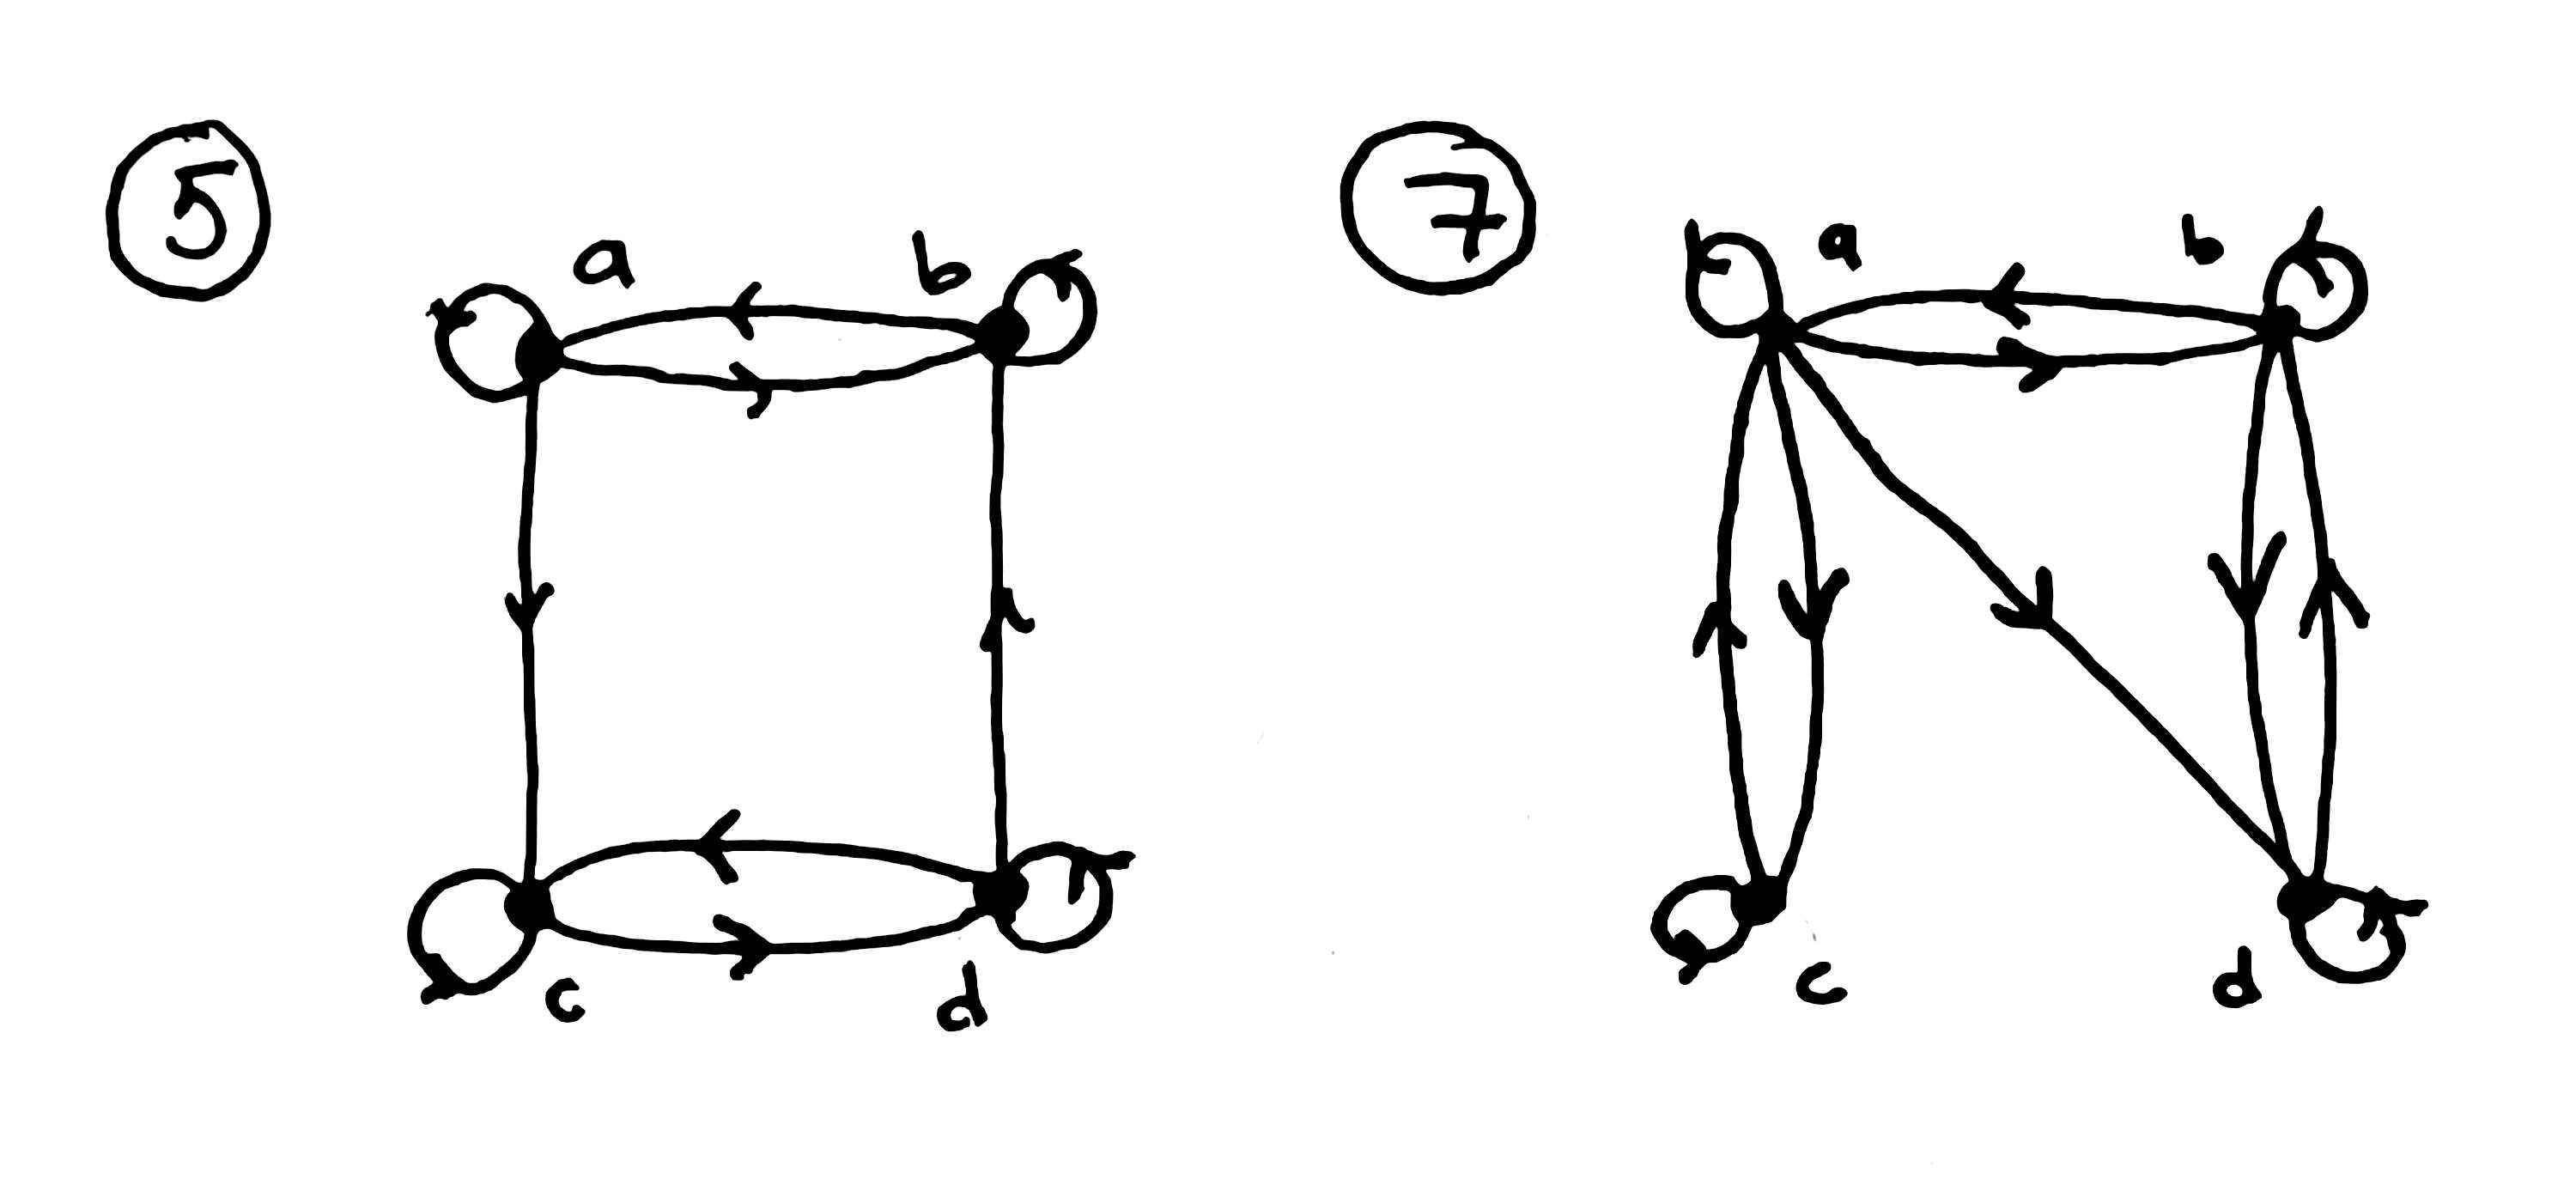
\includegraphics[width=0.8\linewidth]{figures/reflexive.jpg}
\end{center}

\subsection*{9.4.9}
\begin{center}
    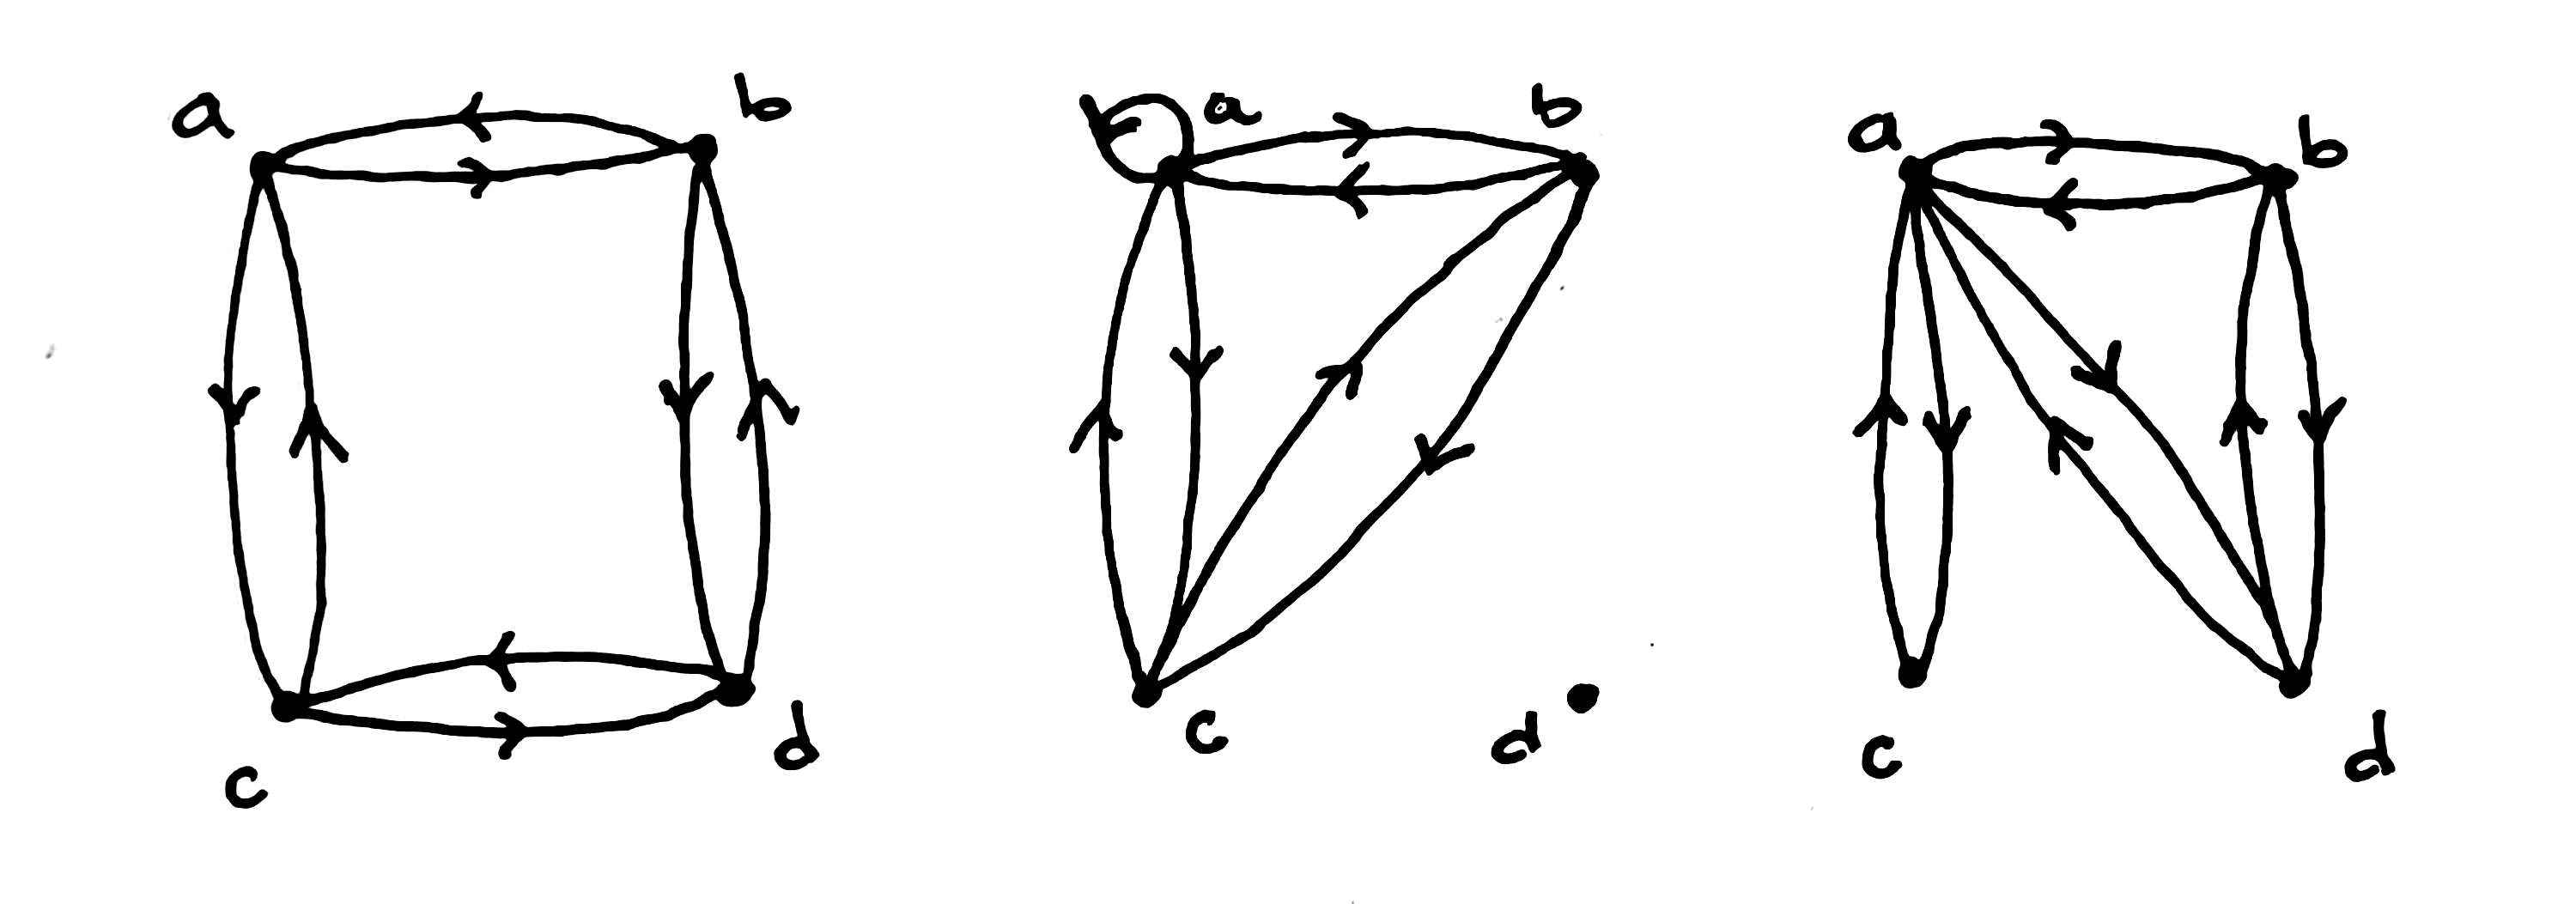
\includegraphics[width=0.8\linewidth]{figures/symmetric.jpg}
\end{center}

\subsection*{9.4.19}
\begin{tasks}
    \task $R^2 = \qty{
        (1,1), (1,5),
        (2,3),
        (3,3), (3,1), (3,2), (3,4),
        (4,1), (4,5),
        (5,3), (5,4)
    }$
    \task $R^3 = \left\{\mqty{
        (1, 1),& (1, 2),& (1, 3),& (1, 4),& \\
        (2, 1),& (2, 5),& \\
        (3, 1),& (3, 3),& (3, 4),& (3, 5),&  \\
        (4, 1),& (4, 2),& (4, 3),& (4, 4),& \\
        (5, 1),& (5, 3),& (5, 5)
    }\right\}$
    \task $R^4 = \left\{\mqty{
        (1, 1),& (1, 3),& (1, 4),& (1, 5),&  \\
        (2, 1),& (2, 2),& (2, 3),& (2, 4),& \\
        (3, 1),& (3, 2),& (3, 3),& (3, 4),& (3, 5),& \\
        (4, 1),& (4, 3),& (4, 4),& (4, 5),& \\
        (5, 1),& (5, 2),& (5, 3),& (5, 4),& (5, 5)
    }\right\}$
    \task $R^5 = \left\{\mqty{
        (1, 1),& (1, 2),& (1, 3),& (1, 4),& (1, 5),& \\
        (2, 1),& (2, 3),& (2, 4),& (2, 5),& \\
        (3, 1),& (3, 2),& (3, 3),& (3, 4),& (3, 5),& \\
        (4, 1),& (4, 2),& (4, 3),& (4, 4),& (4, 5),& \\
        (5, 1),& (5, 2),& (5, 3),& (5, 4),& (5, 5)
    }\right\}$
    \task $R^6 = \left\{\mqty{
        (1, 1),& (1, 2),& (1, 3),& (1, 4),& (1, 5),& \\
        (2, 1),& (2, 2),& (2, 3),& (2, 4),& (2, 5),& \\
        (3, 1),& (3, 2),& (3, 3),& (3, 4),& (3, 5),& \\
        (4, 1),& (4, 2),& (4, 3),& (4, 4),& (4, 5),& \\
        (5, 1),& (5, 2),& (5, 3),& (5, 4),& (5, 5)
    }\right\}$
    \task $R^* = \left\{\mqty{
        (1, 1),& (1, 2),& (1, 3),& (1, 4),& (1, 5),& \\
        (2, 1),& (2, 2),& (2, 3),& (2, 4),& (2, 5),& \\
        (3, 1),& (3, 2),& (3, 3),& (3, 4),& (3, 5),& \\
        (4, 1),& (4, 2),& (4, 3),& (4, 4),& (4, 5),& \\
        (5, 1),& (5, 2),& (5, 3),& (5, 4),& (5, 5)
    }\right\}$
\end{tasks}

\subsection*{9.4.25}
\begin{tasks}(2)
    \task $\mqty[
        1 & 1 & 1 & 1 \\
        1 & 1 & 1 & 1 \\
        1 & 1 & 1 & 1 \\
        1 & 1 & 1 & 1 \\
    ]$
    \task $\mqty[
        0 & 0 & 0 & 0 \\
        1 & 0 & 1 & 1 \\
        1 & 0 & 1 & 1 \\
        1 & 0 & 1 & 1 \\
    ]$
    \task $\mqty[
        0 & 1 & 1 & 1 \\
        0 & 0 & 1 & 1 \\
        0 & 0 & 0 & 1 \\
        0 & 0 & 0 & 0 \\
    ]$
    \task $\mqty[
        1 & 1 & 1 & 1 \\
        1 & 1 & 1 & 1 \\
        1 & 1 & 1 & 1 \\
        1 & 1 & 1 & 1 \\
    ]$
\end{tasks}

\subsection*{9.4.27}
\begin{tasks}(2)
    \task $\mqty[
        1 & 1 & 1 & 1 \\
        1 & 1 & 1 & 1 \\
        1 & 1 & 1 & 1 \\
        1 & 1 & 1 & 1 \\
    ]$
    \task $\mqty[
        0 & 0 & 0 & 0 \\
        1 & 0 & 1 & 1 \\
        1 & 0 & 1 & 1 \\
        1 & 0 & 1 & 1 \\
    ]$
    \task $\mqty[
        0 & 1 & 1 & 1 \\
        0 & 0 & 1 & 1 \\
        0 & 0 & 0 & 1 \\
        0 & 0 & 0 & 0 \\
    ]$
    \task $\mqty[
        1 & 1 & 1 & 1 \\
        1 & 1 & 1 & 1 \\
        1 & 1 & 1 & 1 \\
        1 & 1 & 1 & 1 \\
    ]$
\end{tasks}

\subsection*{9.5.1}
\begin{tasks}(2)
    \task Equivalence relation
    \task Not reflexive and not transitive
    \task Equivalence relation
    \task Not transitive
    \task Not symmetric, not transitive
\end{tasks}

\subsection*{9.5.9}
\subsubsection*{Part A}
\begin{proof}
    Examining if $R$ is an equivalence relation necessitates checking 3 conditions
    \begin{enumerate}
        \item If $x \in A$, note that $f(x) = f(y)$ and therefore $(x,x) \in R$. Hence $R$ is reflexive.
        \item Let $x,y \in A$. If $(x,y) \in R$, then $f(x) = f(y)$. Since equality is symmetric, $(y,x) \in R$ and $R$ is hence symmetric.
        \item Let $x,y,z \in A$ with $(x,y) \in R$ and $(y,z) \in R$. Then $f(x) = f(y)$ and $f(y) = f(z)$. Therefore $f(x) = f(z)$ meaning $(x,z) \in R$. Hence $R$ is transitive.
    \end{enumerate}
    Since $R$ is reflexive, symmetric, and transitive, it is an equivalence relation.
\end{proof}

\subsubsection*{Part B}
Its the set of all pre-images of elements in the co-domain

\subsection*{9.5.27}
\begin{tasks}
    \task The sets of people of the same age 
    \task The sets of people with the same two parents
\end{tasks}

\subsection*{9.6.1}
\begin{tasks}
    \task Partial ordering
    \task Not antisymmetric, not transitive
    \task Partial ordering
    \task Partial ordering
    \task Not antisymmetric, not transitive
\end{tasks}

\subsection*{9.6.7}
\begin{tasks}
    \task Not antisymmetric $\implies$ No
    \task Yes
    \task No transitive $\implies$ No
\end{tasks}

\subsection*{9.6.23}
\begin{center}
    \includesvg[width=0.85\linewidth]{figures/hess.svg}
\end{center}

\subsection*{10.1.1} % TODO
\begin{center}
    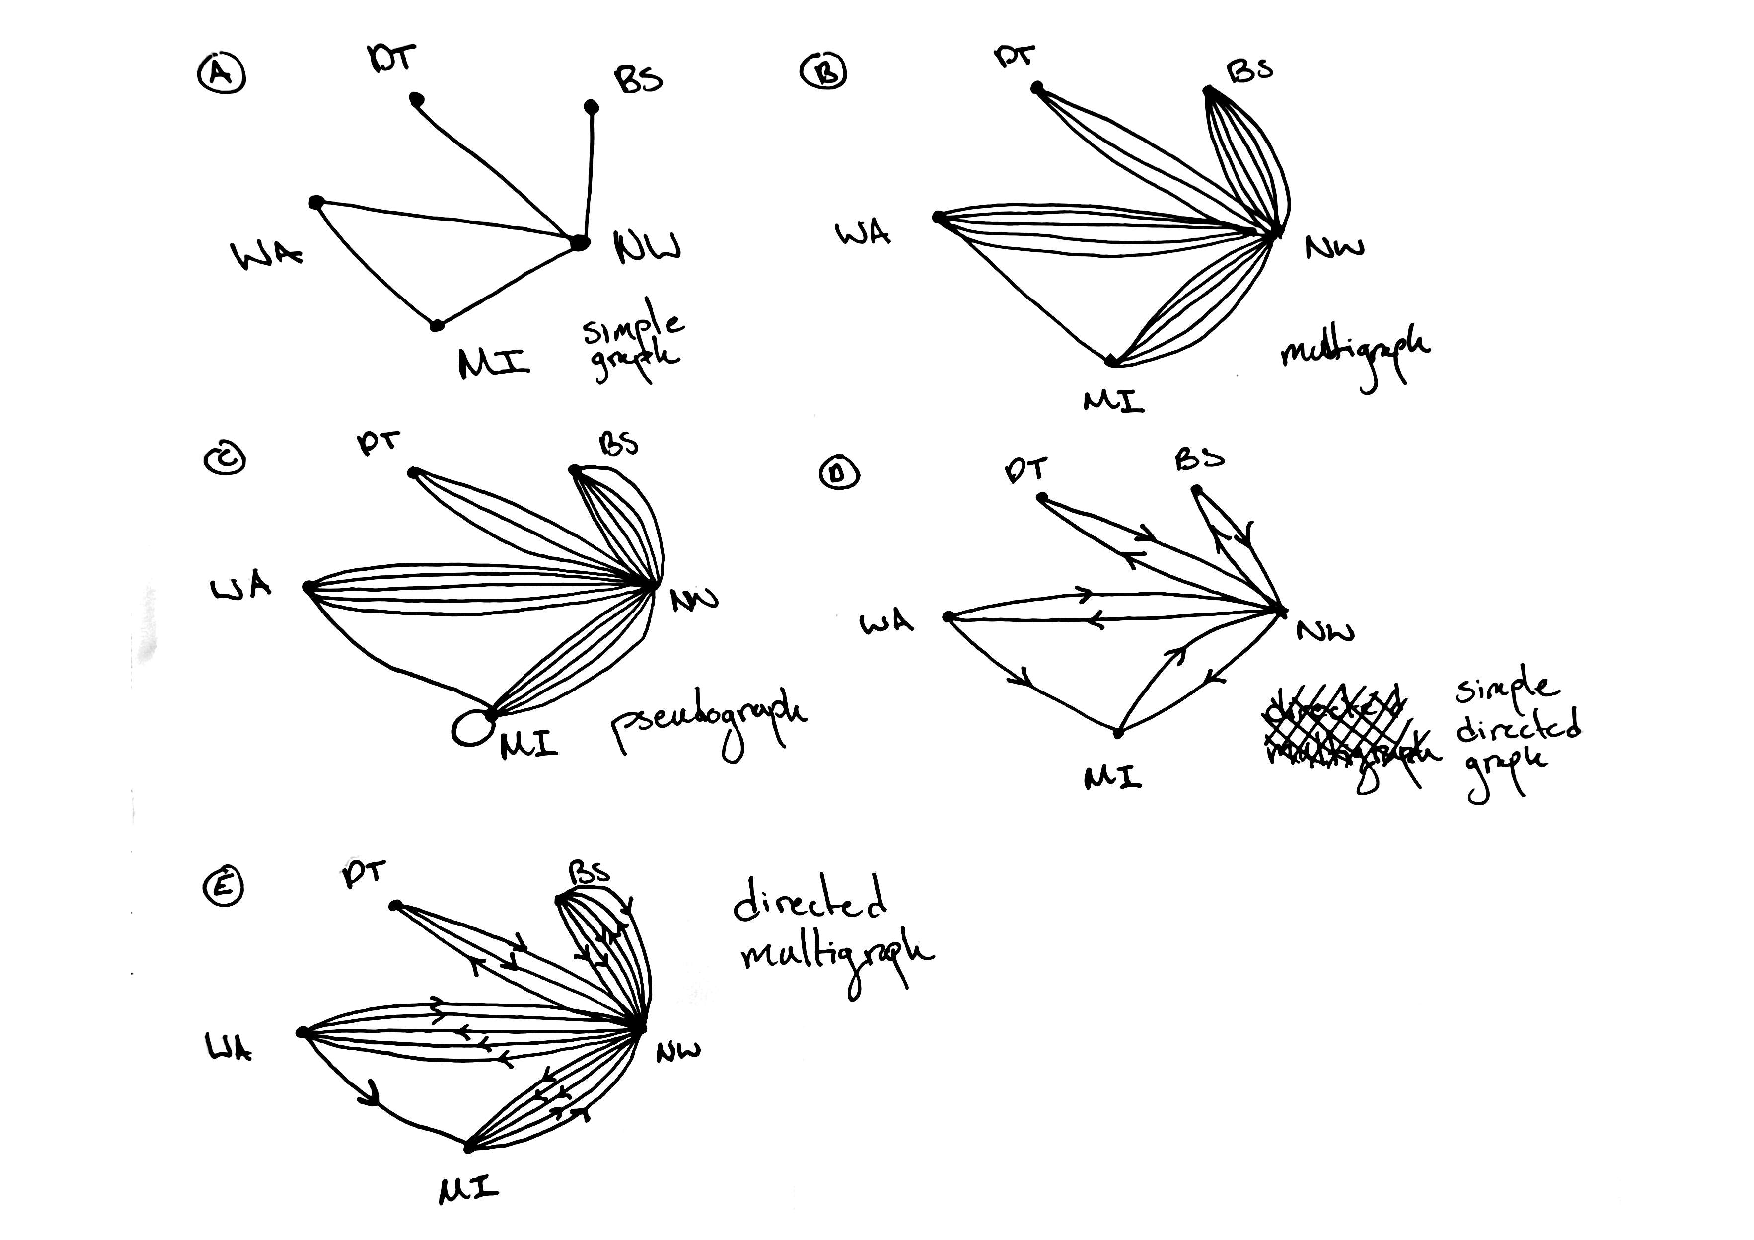
\includegraphics[scale=0.6]{figures/planes.pdf}
\end{center}

\subsection*{10.1.5}
The edges are undirected, there are multiple edges, and there are loops. Therefore the graph is a pseudograph

\subsection*{10.1.9}
The edges are directed, there are multiple edges, and there are loops. Therefore the graph is a directed multigraph.

\end{document}
